% ------------------------------------------------------------------------------
% TYPO3 CMS 7.0 - What's New - Chapter "Deprecated Functions" (English Version)
%
% @author	Michael Schams <schams.net>
% @license	Creative Commons BY-NC-SA 3.0
% @link		http://typo3.org/download/release-notes/whats-new/
% @language	English
% ------------------------------------------------------------------------------
% LTXE-CHAPTER-UID:		4318d159-8d6e71cb-e956516b-17d07fea
% LTXE-CHAPTER-NAME:	Deprecated Functions
% ------------------------------------------------------------------------------

\section{Funzionalità deprecate/rimosse}
\begin{frame}[fragile]
	\frametitle{Funzionalità deprecate/rimosse}

	\begin{center}\huge{Capitolo 5:}\end{center}
	\begin{center}\huge{\color{typo3darkgrey}\textbf{Funzionalità deprecate/rimosse}}\end{center}

\end{frame}

% ------------------------------------------------------------------------------
% LTXE-SLIDE-START
% LTXE-SLIDE-UID:		42f62dc8-a14c1200-683de4ac-bd83ac58
% LTXE-SLIDE-ORIGIN:	c47248f9-03aa1da2-8dd9985d-762cf405 English
% LTXE-SLIDE-TITLE:		Legacy Layer
% LTXE-SLIDE-REFERENCE:	http://typo3.org/news/article/retaining-compatibility-to-typo3-cms6/
% ------------------------------------------------------------------------------

\begin{frame}[fragile]
	\frametitle{Funzionalità deprecate/rimosse}
	\framesubtitle{Layer di compatibilità}

	\begin{itemize}

		\item TYPO3 CMS 6.2: un layer di compatibilità permetteva alle vecchie estensioni di funzionare nel nuovo codice\newline
			\small
				Svantaggi: diminuzione delle prestazioni (non per l'intero sistema)
			\normalsize

		\item TYPO3 CMS 7.0: il layer di compatibilità è stato rimosso dal core\newline
			\small
				Impatto: le vecchie estensioni potrebbero non funzionare (es. estensioni senza namespace)
			\normalsize

		\item La compatibilità può essere forzata installando l'estensione di sistema \texttt{EXT:compatibility6} se necessaria
		\item Questa estensione sarà rimossa dal TER nel futuro

	\end{itemize}

\end{frame}

% ------------------------------------------------------------------------------
% LTXE-SLIDE-START
% LTXE-SLIDE-UID:		80b96ace-7385d36e-1405c6e9-9cad1d8f
% LTXE-SLIDE-ORIGIN:	70da8aab-cd42e15f-fe254b81-41ceabb5 English
% LTXE-SLIDE-TITLE:		Backend User Management
% ------------------------------------------------------------------------------

\begin{frame}[fragile]
	\frametitle{Funzionalità deprecate/rimosse}
	\framesubtitle{Gestione user di backend}

	\begin{itemize}
		\item La funzionalità per cambio utente nel backend ("change-to mode") è stata rimossa
	\end{itemize}

	\smaller\tabto{1cm}\begingroup\color{typo3red}TYPO3 CMS 6.2\endgroup\normalsize
	\begin{figure}\vspace{-0.4cm}
		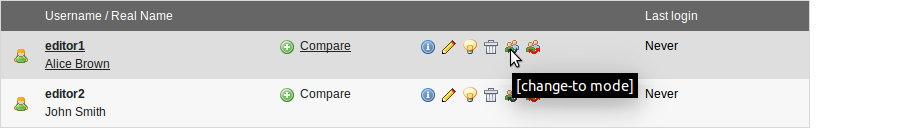
\includegraphics[width=0.90\linewidth]{DeprecatedRemovedFunctions/BackendUserSwitch1.png}
	\end{figure}

	\smaller\tabto{1cm}\begingroup\color{typo3red}TYPO3 CMS 7.0\endgroup\normalsize
	\begin{figure}\vspace{-0.4cm}
		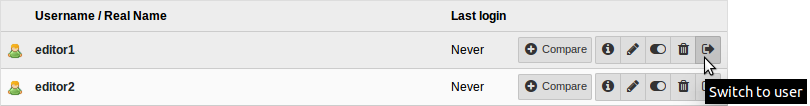
\includegraphics[width=0.90\linewidth]{DeprecatedRemovedFunctions/BackendUserSwitch2.png}
	\end{figure}

\end{frame}

% ------------------------------------------------------------------------------
% LTXE-SLIDE-START
% LTXE-SLIDE-UID:		87794406-e13d8da2-7df80f3f-73c8068c
% LTXE-SLIDE-ORIGIN:	10805d4d-787ce2f8-10e4329a-1451521a English
% LTXE-SLIDE-TITLE:		Removed Deprecated JavaScript Functions
% LTXE-SLIDE-REFERENCE:	https://github.com/TYPO3/TYPO3.CMS/commit/2dff81b963e1b77c7f068f91ffde73914a18b0be
% LTXE-SLIDE-REFERENCE:	https://forge.typo3.org/issues/62291
% LTXE-SLIDE-REFERENCE:	https://forge.typo3.org/projects/typo3cms-core/repository/revisions/9ac03e383e4786e868f4b1d81893e84c4621abc8/entry/typo3/sysext/core/Documentation/Changelog/master/Breaking-62291-RTEDeprecatedJavaScriptMethodsRemoved.rst
% ------------------------------------------------------------------------------

\begin{frame}[fragile]
	\frametitle{Funzionalità deprecate/rimosse}
	\framesubtitle{Rimosse le funzioni deprecate di Javascript}

	\begin{itemize}
		\item In accordo con la \href{http://forge.typo3.org/projects/typo3v4-core/wiki/CoreDevPolicy}{strategia di deprecazione},
			un certo numero di metodi JavaScript, classificati come \textit{deprecati} fin da TYPO3 CMS 4.7, sono stati rimossi, come ad esempio:

		\begin{lstlisting}
			\TYPO3\CMS\Backend\Form\FormEngine->getSingleField_typeInput
			\TYPO3\CMS\Backend\Form\FormEngine->getSingleField_typeText
			\TYPO3\CMS\Core\Utility\GeneralUtility->quoted_printable
			\TYPO3\CMS\Core\Utility\GeneralUtility->encodeHeader
		\end{lstlisting}

		\smaller
			\texttt{HTMLArea.Editor.forceRedraw}\newline
				(usa invece \texttt{HTMLArea.Framework.doLayout})
				\vspace{0.2cm}

			\texttt{HTMLArea.Editor.convertNode}\newline
				(usa invece \texttt{HTMLArea.DOM.convertNode})
				\vspace{0.2cm}

			\texttt{HTMLArea.Editor.getBlockAncestors}\newline
				(usa invece \texttt{HTMLArea.DOM.getBlockAncestors})
		\normalsize

	\end{itemize}

\end{frame}

% ------------------------------------------------------------------------------
% LTXE-SLIDE-START
% LTXE-SLIDE-UID:		5e071728-195f3ae3-af04da89-6b43a9ee
% LTXE-SLIDE-ORIGIN:	9da41efc-970e66a8-f9163c40-67cfa712 English
% LTXE-SLIDE-TITLE:		Removed Functions (1)
% LTXE-SLIDE-REFERENCE:	https://forge.typo3.org/issues/17579
% LTXE-SLIDE-REFERENCE:	https://forge.typo3.org/issues/62888
% ------------------------------------------------------------------------------

\begin{frame}[fragile]
	\frametitle{Funzionalità deprecate/rimosse}
	\framesubtitle{Funzionalità rimosse (1)}

	\begin{itemize}

		\item
			\small
				L'opzione TypoScript \texttt{config.uniqueLinkVars} è stata rimossa\newline
				(questo comportamento è ora un'impostazione predefinita)
			\normalsize

		\item
			\small
				Il ViewHelper
					\texttt{\textbackslash
						TYPO3\textbackslash
						CMS\textbackslash
						Documentation\textbackslash
						ViewHelpers\textbackslash
						Link\textbackslash
						Action}
					è stato rimosso (usa invece \texttt{f:be.buttons.icon} o \texttt{f:uri.*})
			\normalsize

		\item
			\small
				L'opzione PageTSconfig \texttt{mod.web\_list.alternateBgColors}\newline
				è stata rimossa
			\normalsize

		\item
			\small
				PropertyMapper è stato rimosso\newline
				(inclusa l'opzione \texttt{rewrittenPropertyMapper = 0})
			\normalsize

		\item
			\small
				Le seguenti condizioni TypoScript sono state rimosse:

					\begin{itemize}
						\item\texttt{browser}
						\item\texttt{version}
						\item\texttt{system}
						\item\texttt{useragent}
					\end{itemize}
			\normalsize

	\end{itemize}

\end{frame}

% ------------------------------------------------------------------------------
% LTXE-SLIDE-START
% LTXE-SLIDE-UID:		005723aa-851f261e-9c90c6a3-a4c4f343
% LTXE-SLIDE-ORIGIN:	efe86631-b6020ae8-ffa01160-6de29dc3 English
% LTXE-SLIDE-TITLE:		Removed Functions (1)
% ------------------------------------------------------------------------------

\begin{frame}[fragile]
	\frametitle{Funzionalità deprecate/rimosse}
	\framesubtitle{Metodi rimossi (1)}

	I seguenti \textbf{metodi} sono stati rimossi:

	\begin{itemize}
		\item
			\small
				\texttt{connectDB}\newline
				nella classe
				\texttt{\textbackslash
					TYPO3\textbackslash
					CMS\textbackslash
					Frontend\textbackslash
					Utility\textbackslash
					EidUtility}
			\normalsize
		\item
			\small
				\texttt{isDisplayCondition}\newline
				nella classe
				\texttt{\textbackslash
					TYPO3\textbackslash
					CMS\textbackslash
					Form\textbackslash
					FormEngine}
			\normalsize
		\item
			\small
				\texttt{int\_from\_ver}\newline
				nella classe
				\texttt{\textbackslash
					TYPO3\textbackslash
					CMS\textbackslash
					Core\textbackslash
					Utility\textbackslash
					GeneralUtility}
			\normalsize
		\item
			\small
				\texttt{getUniqueFields}\newline
				nella classe
				\texttt{\textbackslash
					TYPO3\textbackslash
					CMS\textbackslash
					Core\textbackslash
					DataHandling\textbackslash
					DataHandler}
			\normalsize

	\end{itemize}

\end{frame}

% ------------------------------------------------------------------------------
% LTXE-SLIDE-START
% LTXE-SLIDE-UID:		4756f235-e9d64abc-c34584fc-92f28d59
% LTXE-SLIDE-ORIGIN:	293414d4-e87db3d5-afced471-ca9826ed English
% LTXE-SLIDE-TITLE:		Removed Methods (2)
% ------------------------------------------------------------------------------

\begin{frame}[fragile]
	\frametitle{Funzionalità deprecate/rimosse}
	\framesubtitle{Metodi rimossi (2)}

	I seguenti \textbf{metodi} sono stati rimossi:

	\begin{itemize}

		\item
			\small
				\texttt{isSafeModeEnabled}\newline
				nella classe
				\texttt{\textbackslash
					TYPO3\textbackslash
					CMS\textbackslash
					Core\textbackslash
					Utility\textbackslash
					PhpOptionsUtility}
			\normalsize
		\item
			\small
				\texttt{registerSwiftMailer}\newline
				nella classe
				\texttt{\textbackslash
					TYPO3\textbackslash
					CMS\textbackslash
					Core\textbackslash
					Bootstrap}
			\normalsize
		\item
			\small
				\texttt{loadTCA}\newline
				nella classe
				\texttt{\textbackslash
					TYPO3\textbackslash
					CMS\textbackslash
					Core\textbackslash
					Utility\textbackslash
					GeneralUtility}
			\normalsize
		\item
			\small
				\texttt{isLocalconfWritable}\newline
				nella classe
				\texttt{\textbackslash
					TYPO3\textbackslash
					CMS\textbackslash
					Core\textbackslash
					Utility\textbackslash
					ExtensionManagementUtility}
			\normalsize

	\end{itemize}

\end{frame}

% ------------------------------------------------------------------------------
% LTXE-SLIDE-START
% LTXE-SLIDE-UID:		ecaa3e21-801cbfe0-9f083482-ad583624
% LTXE-SLIDE-ORIGIN:	a1ba1998-f88c1063-71470741-30b9f314 English
% LTXE-SLIDE-TITLE:		Removed Classes
% ------------------------------------------------------------------------------

\begin{frame}[fragile]
	\frametitle{Funzionalità deprecate/rimosse}
	\framesubtitle{Classi rimosse}

	Le seguenti \textbf{classi} sono state rimosse:

	\begin{itemize}

		\item
			\smaller
				\texttt{\textbackslash
					TYPO3\textbackslash
					CMS\textbackslash
					Backend\textbackslash
					Template\textbackslash
					MediumDocumentTemplate}
			\normalsize
		\item
			\smaller
				\texttt{\textbackslash
					TYPO3\textbackslash
					CMS\textbackslash
					Extbase\textbackslash
					Service\textbackslash
					TypeHandlingService}
			\normalsize

	\end{itemize}

\end{frame}

% ------------------------------------------------------------------------------
